% !TeX root = ../main.tex
\section{Простейшие типы уравнений первого порядка}

\task{С. 1:13}{Дифференциальное уравнение семейства}
\sourcepage{2}
Дано семейство $x^2=(C+y)e^y$. Требуется исключить $C$.
Дифференцируем по $x$, считая $C$ постоянной:
\[
 2x=(C+y+1)e^y y'.
\]
Из исходного равенства $(C+y)e^y=x^2$, поэтому
\[
 2x=(x^2+e^y)y'.
\]
\answer{$\displaystyle y'=\frac{2x}{x^2+e^y}$. Знаменатель строго положителен.}
Обратно, вдоль любого решения производная $x^2e^{-y}-y$ равна нулю,
так что получено именно заданное семейство.

\task{С. 2:7}{Разделение переменных}
\sourcepage{2--3}
\[
 yy'\cos x=(1-y)\sin x.
\]
Постоянная $y\equiv1$ является решением. При $y\ne1$ и $\cos x\ne0$
\[
 \frac{y}{1-y}\dd y=\tan x\dd x,
 \qquad -y-\ln|1-y|=-\ln|\cos x|+C.
\]
Здесь $y/(1-y)=1/(1-y)-1$. После потенцирования и учёта знаков
\answer{$(1-y)e^y=C\cos x$. Значение $C=0$ даёт $y\equiv1$.}
Формула описывает гладкие ветви исходного уравнения. При $y=0$ нужно
проверять исходное равенство: оно требует $\sin x=0$. Через точку
$\cos x=0$ возможна гладкая ветвь с $y=1$; запрет $\cos x\ne0$ относится
к шагу разделения, а не ко всем решениям. В такой точке $F_y=-e\ne0$
для $F=(1-y)e^y-C\cos x$, так что неявная формула действительно продолжается.

\task{С. 2:10}{Уравнение в дифференциалах}
\sourcepage{3}
\[
 x(y+1)\dd y=(1-y^2)\dd x.
\]
Переносим всё в одну сторону и выносим общий множитель:
\[
 (y+1)\bigl[x\dd y+(y-1)\dd x\bigr]=0.
\]
Поэтому либо $y\equiv-1$, либо $\dd[x(y-1)]=0$.
\answer{$x(1-y)=C$ и $y\equiv-1$. При $x\ne0$ первое семейство имеет вид
$y=1-C/x$; $C=0$ даёт $y\equiv1$. Вертикальная прямая $x=0$ также
является интегральной кривой дифференциальной формы.}
Через $x=0$ из первого семейства гладко продолжается только $y\equiv1$.
Склейка непостоянной ветви с $y=-1$ невозможна в классе $C^1$:
в точке пересечения $x_0\ne0$ её производная равна $2/x_0$, а не нулю.

\task{С. 2:44}{Ортогональные траектории}
\sourcepage{4}
Дано $y(1+Ce^x)=1$. Дифференцируя и используя $Ce^x=1/y-1$, получаем
\[
 \frac{y'}y+1-y=0,\qquad y'=y(y-1).
\]
У ортогональной траектории произведение конечных ненулевых угловых
коэффициентов равно $-1$. Поэтому
\[
 \frac{\dd y}{\dd x}=-\frac1{y(y-1)},
 \qquad \frac{\dd x}{\dd y}=y-y^2.
\]
Последняя запись удобна и в точках вертикальной касательной.
\answer{$\displaystyle x=\frac{y^2}{2}-\frac{y^3}{3}+C$.}
Проверка: касательные векторы $(1,y(y-1))$ исходной кривой
и $(y-y^2,1)$ найденной траектории имеют нулевое скалярное произведение.
Сама исходная семья не содержит точек с $y=0$.

\task{№ 55 в рукописи}{Неединственность задачи Коши}
\sourcepage{4--5}
\[
 y'=3\sqrt[3]{y^2}=3|y|^{2/3},\qquad y(2)=0.
\]
При $y\ne0$ разделение даёт $\sqrt[3]y=x-C$, то есть $y=(x-C)^3$.
Кроме того, $y\equiv0$ --- решение. Но перечислить только эти две
возможности недостаточно: к нулевому участку можно присоединить кубические ветви.
\answer{Все максимальные решения задачи задаются на $\R$ формулой
\[
 y(x)=\begin{cases}
 (x-a)^3,&x<a,\\
 0,&a\le x\le b,\\
 (x-b)^3,&x>b,
 \end{cases}\qquad -\infty\le a\le2\le b\le+\infty.
\]
При бесконечном конце соответствующая кубическая ветвь отсутствует.}
В точках склейки и значение, и производная кубической ветви равны нулю.
Полнота следует из $y'\ge0$: множество нулей непрерывного неубывающего
решения является интервалом, а на каждом ненулевом участке
$(\sqrt[3]y)'=1$. Частные случаи: $a=b=2$ даёт $(x-2)^3$,
$a=-\infty$, $b=+\infty$ даёт нулевое решение.
\editnote{Номер 55 сохранён по рукописи. В приложенном издании сборника
С.\,2:55 имеет другую формулировку; здесь решено именно выписанное уравнение.}

\task{Ф. 62}{Замена разности переменных}
\sourcepage{5--6}
\[
 y'=\cos(y-x).
\]
Положим $z=y-x$. Тогда $z'=\cos z-1=-2\sin^2(z/2)$.
Равновесия $z=2\pi k$ дают $y=x+2\pi k$. На остальных ветвях
\[
 \int\frac{\dd z}{-2\sin^2(z/2)}=x+C,
 \qquad \cot\frac z2=x+C.
\]
\answer{$\displaystyle \cot\frac{y-x}{2}=x+C$ либо $y=x+2\pi k$, $k\in\Z$.}
Можно выразить непостоянные ветви явно:
$y=x+2\arccot(x+C)+2\pi k$, где $\arccot\colon\R\to(0,\pi)$.
Все эти решения определены на $\R$; периодические сдвиги нельзя
потерять при обращении котангенса.
\begin{center}
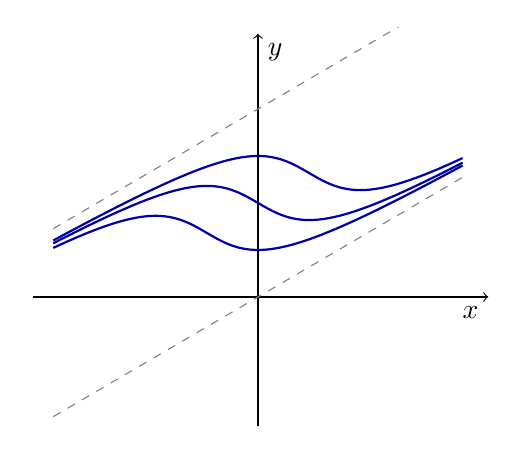
\begin{tikzpicture}[x=.65cm,y=.38cm]
 \clip (-4.5,-4.5) rectangle (4.7,9);
 \draw[->] (-4.4,0)--(4.5,0) node[below left] {$x$};
 \draw[->] (0,-4.3)--(0,8.8) node[below right] {$y$};
 \draw[dashed,gray,domain=-4:4] plot(\x,\x);
 \draw[dashed,gray,domain=-4:4] plot(\x,{\x+2*pi});
 \foreach \c in {-1,0,1}{
  \draw[thick,blue!65!black,domain=-4:4,samples=100]
    plot(\x,{\x+pi-2*atan(\x+\c)*pi/180});}
\end{tikzpicture}
\end{center}
На рисунке показаны три непостоянные ветви и прямые $y=x$, $y=x+2\pi$.
У непостоянных ветвей есть участки убывания: из явной формулы
$y'=1-2/(1+(x+C)^2)$, поэтому схематический монотонный рисунок
в рукописи здесь уточнён.

\task{С. 2:59}{Однородное уравнение с корнем}
\sourcepage{6--7}
\[
 x\dd y=(y+\sqrt{x^2+y^2})\dd x,\qquad x\ge0.
\]
При $x>0$ положим $z=y/x$. Тогда $y'=z+xz'$ и
\[
 xz'=\sqrt{1+z^2},\qquad
 \ln\bigl(z+\sqrt{1+z^2}\bigr)=\ln x+C.
\]
Левая скобка положительна, поэтому после потенцирования
\[
 z+\sqrt{1+z^2}=Ax,\quad A=e^C>0,
 \qquad y+\sqrt{x^2+y^2}=Ax^2.
\]
Выражая $y$ (или используя $\sinh(\ln(Ax))$), получаем
\answer{$\displaystyle y=\frac{Ax^2}{2}-\frac1{2A}$, $A>0$, $x>0$.}
Такая ветвь гладко доходит до $x=0$ со значением $-1/(2A)$ и
удовлетворяет исходному равенству на границе. Для дифференциальной
формы отдельно имеется вертикальная интегральная кривая $x=0$.
\editnote{В рукописи константа после потенцирования ошибочно допускает
оба знака. Отрицательные значения не удовлетворяют исходному уравнению с корнем.}

\task{С. 2:73}{Сдвиг начала координат}
\sourcepage{7--8}
\[
 (2x-y-2)\dd x+(x+y-4)\dd y=0.
\]
Прямые $2x-y-2=0$ и $x+y-4=0$ пересекаются в $(2,2)$.
В координатах $X=x-2$, $Y=y-2$ уравнение становится однородным:
\[
 (2X-Y)\dd X+(X+Y)\dd Y=0.
\]
При $X\ne0$ вводим $t=Y/X$, $\dd Y=t\dd X+X\dd t$:
\[
 X(2+t^2)\dd X+X^2(1+t)\dd t=0,
 \qquad -\frac{\dd X}{X}=\frac{1+t}{2+t^2}\dd t.
\]
Интегрирование даёт
\[
 \ln|X|+\tfrac12\ln(2+t^2)+\tfrac1{\sqrt2}\arctan\frac t{\sqrt2}=C.
\]
\answer{Локально при $x\ne2$:
\[
 \ln\bigl(2(x-2)^2+(y-2)^2\bigr)
 +\sqrt2\arctan\frac{y-2}{\sqrt2(x-2)}=C.
\]}
Прямая $x=2$ не является отдельной интегральной кривой, однако решения
могут её пересекать. Для продолжения следует понимать арктангенс как
непрерывный угол $\theta=\arg(\sqrt2X+iY)$ вдоль кривой:
$\ln(2X^2+Y^2)+\sqrt2\theta=C$.
Это устраняет искусственный разрыв выбранной ветви арктангенса.
Через центр $(2,2)$ нет $C^1$-графика решения: если
$Y=mX+o(X)$, подстановка в уравнение для графика даёт $2+m^2=0$.

\task{С. 2:80}{Задача Коши для однородного уравнения}
\sourcepage{8--9}
\[
 y'=\frac{y-2x}{x+2y},\qquad y(1)=0.
\]
Вблизи начальной точки $x>0$. Подстановка $t=y/x$ приводит к
\[
 x(1+2t)t'=-2(1+t^2),\qquad
 \ln(1+t^2)+\arctan t=-2\ln x+C.
\]
Начальное условие даёт $C=0$.
\answer{Вблизи $(1,0)$: $\displaystyle x^2+y^2=e^{-\arctan(y/x)}$.}
Для описания всего непродолжаемого графика удобно взять полярный угол:
\[
 x=e^{-\theta/2}\cos\theta,\qquad
 y=e^{-\theta/2}\sin\theta,
 \qquad -\arctan\tfrac12<\theta<\pi-\arctan\tfrac12.
\]
Действительно, $x+2y=e^{-\theta/2}(\cos\theta+2\sin\theta)$ не равен
нулю внутри этого промежутка, а $\dd x/\dd\theta=-(x+2y)/2<0$.
Поэтому параметризация задаёт однозначный график на интервале
\[
 -\frac2{\sqrt5}e^{-(\pi-\alpha)/2}<x<
 \frac2{\sqrt5}e^{\alpha/2},\qquad \alpha=\arctan\tfrac12.
\]
На концах обращается в нуль знаменатель исходного уравнения.
Формулу с главным значением $\arctan(y/x)$ нельзя без смены ветви
использовать после пересечения $x=0$.

\task{С. 3:25}{Линейное уравнение}
\sourcepage{9}
\[
 xy'-3y=4x^2.
\]
При $x\ne0$ умножаем $y'-3y/x=4x$ на $x^{-3}$:
\[
 \left(\frac{y}{x^3}\right)'=\frac4{x^2},\qquad
 \frac{y}{x^3}=-\frac4x+C.
\]
\answer{$y=Cx^3-4x^2$.}
У исходного уравнения в точке $x=0$ требуется $y(0)=0$.
Если нужен график на интервале через нуль, константы $C_-$ и $C_+$
слева и справа могут различаться: полученная функция всё равно имеет
непрерывную первую (и даже вторую) производную и удовлетворяет уравнению.

\task{С. 3:59}{Уравнение Бернулли}
\sourcepage{9--10}
\[
 xy'-y+4y^3=0.
\]
Сначала сохраняем решение $y\equiv0$. Для $x\ne0$, $y\ne0$
полагаем $z=y^{-2}$, откуда $z'=-2y^{-3}y'$ и
\[
 z'+\frac2x z=\frac8x,\qquad (x^2z)'=8x.
\]
Таким образом, $z=4+C/x^2$.
\answer{$y\equiv0$ либо $\displaystyle y^{-2}=4+\frac C{x^2}$,
то есть $\displaystyle y=\frac{\varepsilon}{\sqrt{4+C/x^2}}$,
$\varepsilon\in\{-1,1\}$, на интервалах $x\ne0$, $4+C/x^2>0$.}
При $C=0$ получаются также постоянные $y=\pm\tfrac12$.
Через нуль непостоянные ветви продолжаются в виде
$y=ax/\sqrt{1+4a^2x^2}$; вместе с постоянными $\pm\tfrac12$
это даёт все $C^1$-решения в окрестности нуля. Здесь $a=y'(0)$,
а $a=0$ даёт нулевое решение.

\task{С. 3:68}{Выбор независимой переменной}
\sourcepage{10--11}
\[
 y\dd x+(2x^2y-3x)\dd y=0.
\]
Оси $y=0$ и $x=0$ являются интегральными кривыми формы.
Для остальных ветвей выгоднее считать $x=x(y)$:
\[
 \frac{\dd x}{\dd y}-\frac3y x=-2x^2.
\]
Подстановка $u=1/x$ даёт линейное уравнение
\[
 u'+\frac3y u=2,\qquad (y^3u)'=2y^3,
 \qquad \frac{y^3}{x}=\frac{y^4}{2}+C.
\]
\answer{$y^3(xy-2)=Cx$, а также вертикальная кривая $x=0$.}
При $C=0$ первое равенство содержит $y=0$ и $xy=2$.
На ненулевых ветвях выделяются участки, являющиеся графиками $y(x)$;
там, где $2x^2y-3x=0$ и $y\ne0$, конечной производной $y'$ нет.
Метод с $u=1/x$ заменяет более длинную цепочку двух замен из рукописи.

\task{С. 3:94}{Уравнение Риккати}
\sourcepage{12--13}
\[
 x^2y'-5xy+x^2y^2+8=0.
\]
При $x=0$ уравнение невозможно, поэтому $x\ne0$.
Подстановка $y_0=2/x$ даёт $-2-10+4+8=0$.
Положим $y=2/x+z$. После раскрытия скобок:
\[
 z'-\frac zx+z^2=0.
\]
При $z\ne0$ вводим $u=1/z$:
\[
 u'+\frac ux=1,\qquad (xu)'=x,\qquad
 u=\frac x2+\frac Cx.
\]
\answer{$\displaystyle y=\frac2x+\frac{2x}{x^2+C}$,
$x\ne0$, $x^2+C\ne0$, а также $\displaystyle y=\frac2x$.}

\task{Ф. 146}{Линейное уравнение для обратной функции}
\sourcepage{13--14}
\[
 (2e^y-x)y'=1.
\]
Производная решения нигде не равна нулю. Поэтому локально допустима
обратная функция $x=x(y)$, для которой
\[
 \frac{\dd x}{\dd y}+x=2e^y,
 \qquad \frac{\dd}{\dd y}(xe^y)=2e^{2y}.
\]
\answer{$x=e^y+Ce^{-y}$. Для графика $y(x)$ выбирают ветвь,
на которой $\dd x/\dd y=e^y-Ce^{-y}\ne0$.}
Если $C>0$, точка $e^{2y}=C$ не принадлежит графику решения исходного
уравнения: в ней коэффициент при $y'$ равен нулю, а правая часть равна единице.

\task{С. 4:4}{Полный дифференциал}
\sourcepage{14}
\[
 (y-\sin x)\dd x+(x+e^y)\dd y=0.
\]
Для $P=y-\sin x$, $Q=x+e^y$ имеем $P_y=Q_x=1$.
Непосредственно группируем слагаемые:
\[
 y\dd x+x\dd y-\sin x\dd x+e^y\dd y
 =\dd(xy+\cos x+e^y).
\]
\answer{$xy+\cos x+e^y=C$.}

\task{С. 4:20}{Интегрирующий множитель}
\sourcepage{14--15}
\[
 2xy\dd x-(x^2-2y^3)\dd y=0.
\]
Отдельно сохраняем $y\equiv0$. Ищем множитель $\mu=\mu(y)$.
Из условия $(\mu P)_y=(\mu Q)_x$ следует
\[
 \frac{\mu'}\mu=\frac{Q_x-P_y}{P}=-\frac2y,
 \qquad \mu=y^{-2}.
\]
Хотя отношение было записано при $P\ne0$, полученный множитель
проверяется напрямую при любом $x$ и $y\ne0$:
\[
 \frac{2x}{y}\dd x-\frac{x^2}{y^2}\dd y+2y\dd y
 =\dd\left(\frac{x^2}{y}+y^2\right)=0.
\]
\answer{$\displaystyle \frac{x^2}{y}+y^2=C$, $y\ne0$, а также $y\equiv0$.}
Для продолжения к $y=0$ удобно записать $x^2+y^3=Cy$.
Каждая гладкая ветвь этого равенства удовлетворяет исходному уравнению,
в том числе при переходе через $(0,0)$: умножение его дифференциала
на $y$ с последующим использованием $Cy=x^2+y^3$ даёт исходную форму.
Например, при $C\ne0$ теорема о неявной функции даёт гладкую ветвь
$y=x^2/C+o(x^2)$ через начало координат.

\task{С. 4:59}{Замена суммы квадратов}
\sourcepage{15}
\[
 x^2yy'+x^3=(x^2+y^2)^2.
\]
Положим $z=x^2+y^2$. Тогда $z'=2x+2yy'$ и при $x\ne0$
\[
 \frac{x^2}{2}z'=z^2,\qquad
 -\frac1z=-\frac2x+C.
\]
Здесь $z>0$ при $x\ne0$, поэтому деление на $z$ не теряет решений.
\answer{$x=(2+Cx)(x^2+y^2)$, или
$\displaystyle y^2=\frac{x}{2+Cx}-x^2$, на гладких вещественных ветвях.}
Необходимо $2+Cx\ne0$. Точка $x=0$ потребовала бы $y=0$,
но $C^1$-продолжение туда невозможно: если $y(0)=0$ и $y'$ ограничена,
то $z=O(x^2)$, что противоречит $z=x/(2+Cx)\sim x/2$.
В точке $y=0$ при $x\ne0$ исходное уравнение требует $x=1$;
обычный выбор знака квадратного корня не гарантирует гладкости в таком нуле.
Например, при $C=-1$ гладкие ветви через $(1,0)$ записываются как
$y=\pm(x-1)\sqrt{x/(2-x)}$, $0<x<2$, а не с модулем $|x-1|$.

\task{Д. 1}{Риккати с известным частным решением}
\sourcepage{16}
\[
 y'=\frac{y^2}{x^4}-\frac{2y}{x}+4x^2,\qquad x\ne0.
\]
Проверяем частное решение $y_0=x^3$: обе части равны $3x^2$.
Подстановка $z=y-x^3$ даёт $z'=z^2/x^4$.
При $z\ne0$ интегрируем:
\[
 -\frac1z=-\frac1{3x^3}+C.
\]
\answer{$\displaystyle \frac1{y-x^3}=\frac1{3x^3}+C$,
а также $y=x^3$. В явном виде непостоянное по $z$ семейство:
$\displaystyle y=x^3+\frac{3x^3}{1+3Cx^3}$; нули знаменателя исключаются.}
